% !TEX root = ../../main.tex
\section{Central direction from constant areal speed}

\subsection{3.1 Newton's area-law centripetal direction}
\label{subsec:central-direction}

We briefly recall Newton's original geometric implication of Kepler's area law (1609) in the \emph{Principia} (Book~I, Proposition~1, 1687) \cite{newton1687principia}. We do not repeat Newton's elementary geometric proof here; an accessible modern retelling is in Section~22 (``The Area Theorem'') of Chapter~5 of \cite{chandrasekhar1995principia}. A short online exposition in the same geometric spirit is also available in \cite{nonagonnewtonkepler}, and a detailed fill-in of some steps in Newton's Proposition~1 is given in \cite{nauenberg2003keplerarea}.

\begin{figure}[t]
  \centering
  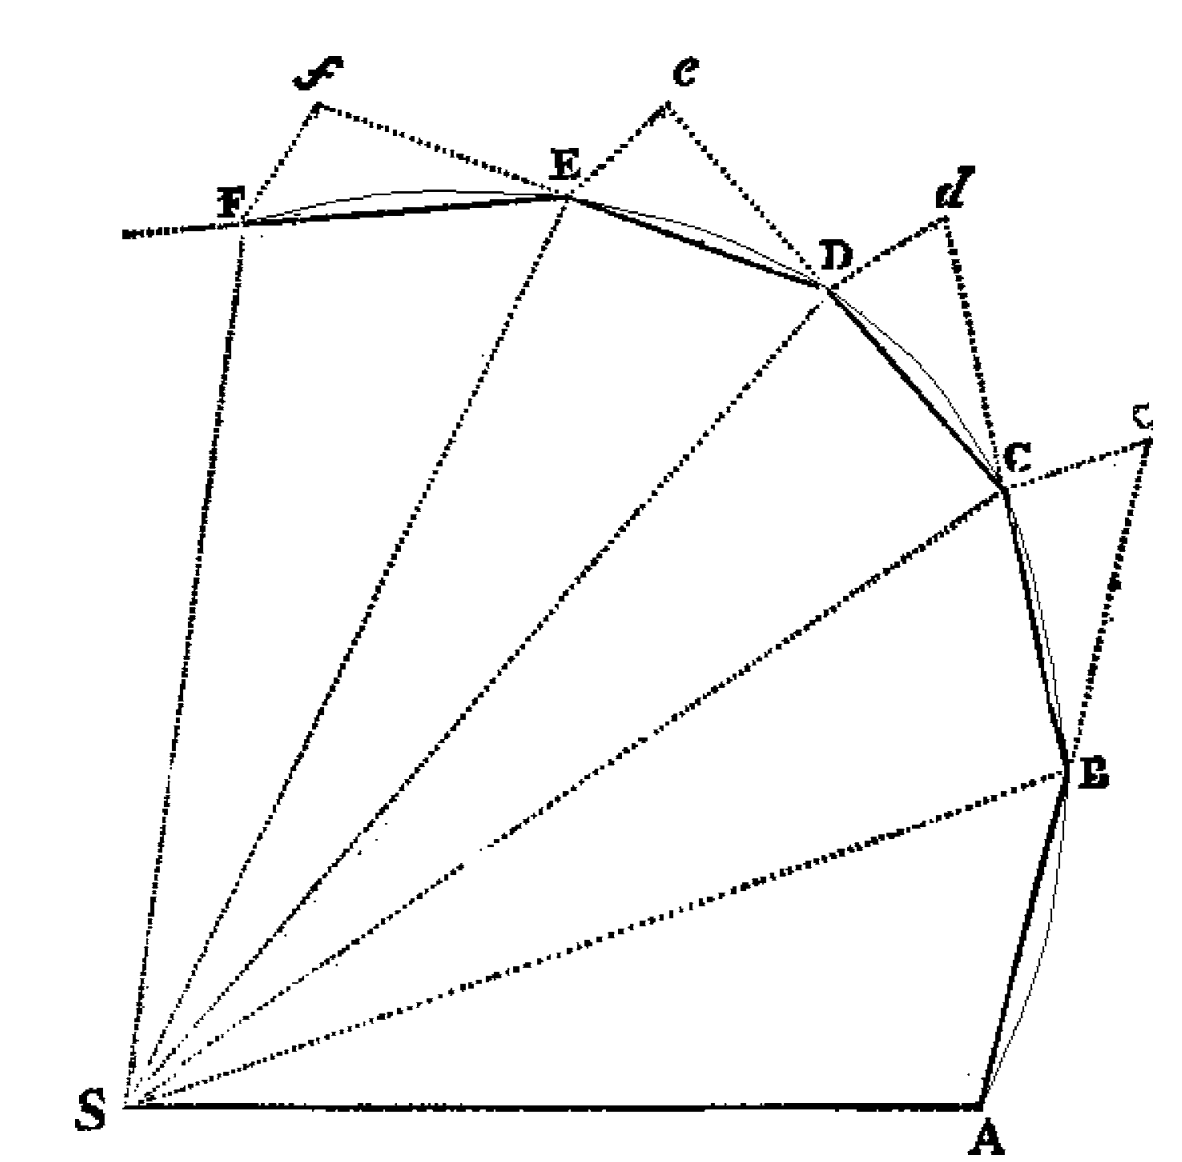
\includegraphics[width=0.5\linewidth]{assets/images/newtonArea.png}
  \caption{Newton's area theorem construction, reproduced from \cite{newton1687principia}. Because it is an original 1687 diagram, it naturally looks coarse/ancient, but the geometric idea is clear.}
  \label{fig:newton-area}
\end{figure}

Approximate the orbit by a broken line $ABCDEF\cdots$ traversed in equal time steps, with instantaneous ``impulses'' at the vertices. Fix the point $S$ about which areas are swept. If there is no impulse at $B$, then after $AB$ the motion would continue straight to a point $c$ on the extension of $AB$ with $Bc=AB$. Newton's construction draws through $c$ a line parallel to $SB$ and places $C$ on this line so that $C\in SC$ (see \Cref{fig:newton-area}); this makes the successive swept triangles $\triangle SAB$ and $\triangle SBC$ have equal areas. Conversely, if equal areas are swept in equal times, then at each vertex the ``jump'' from the straight continuation (e.g., from $c$ back to $C$) must lie along $BS$ (and similarly at $C,D,\ldots$). In the smooth limit, the acceleration is therefore always directed along $AS$, i.e., the force is \emph{centripetal} with center $S$.

Thus it remains to determine the magnitude of the centripetal acceleration $a(r)$.

\subsection{Local distance relationships for \texorpdfstring{$BD$ and $BR^2$}{BD and BR squared}}
\label{subsec:central-direction-lemmas}

\begin{figure}[t]
  \centering
  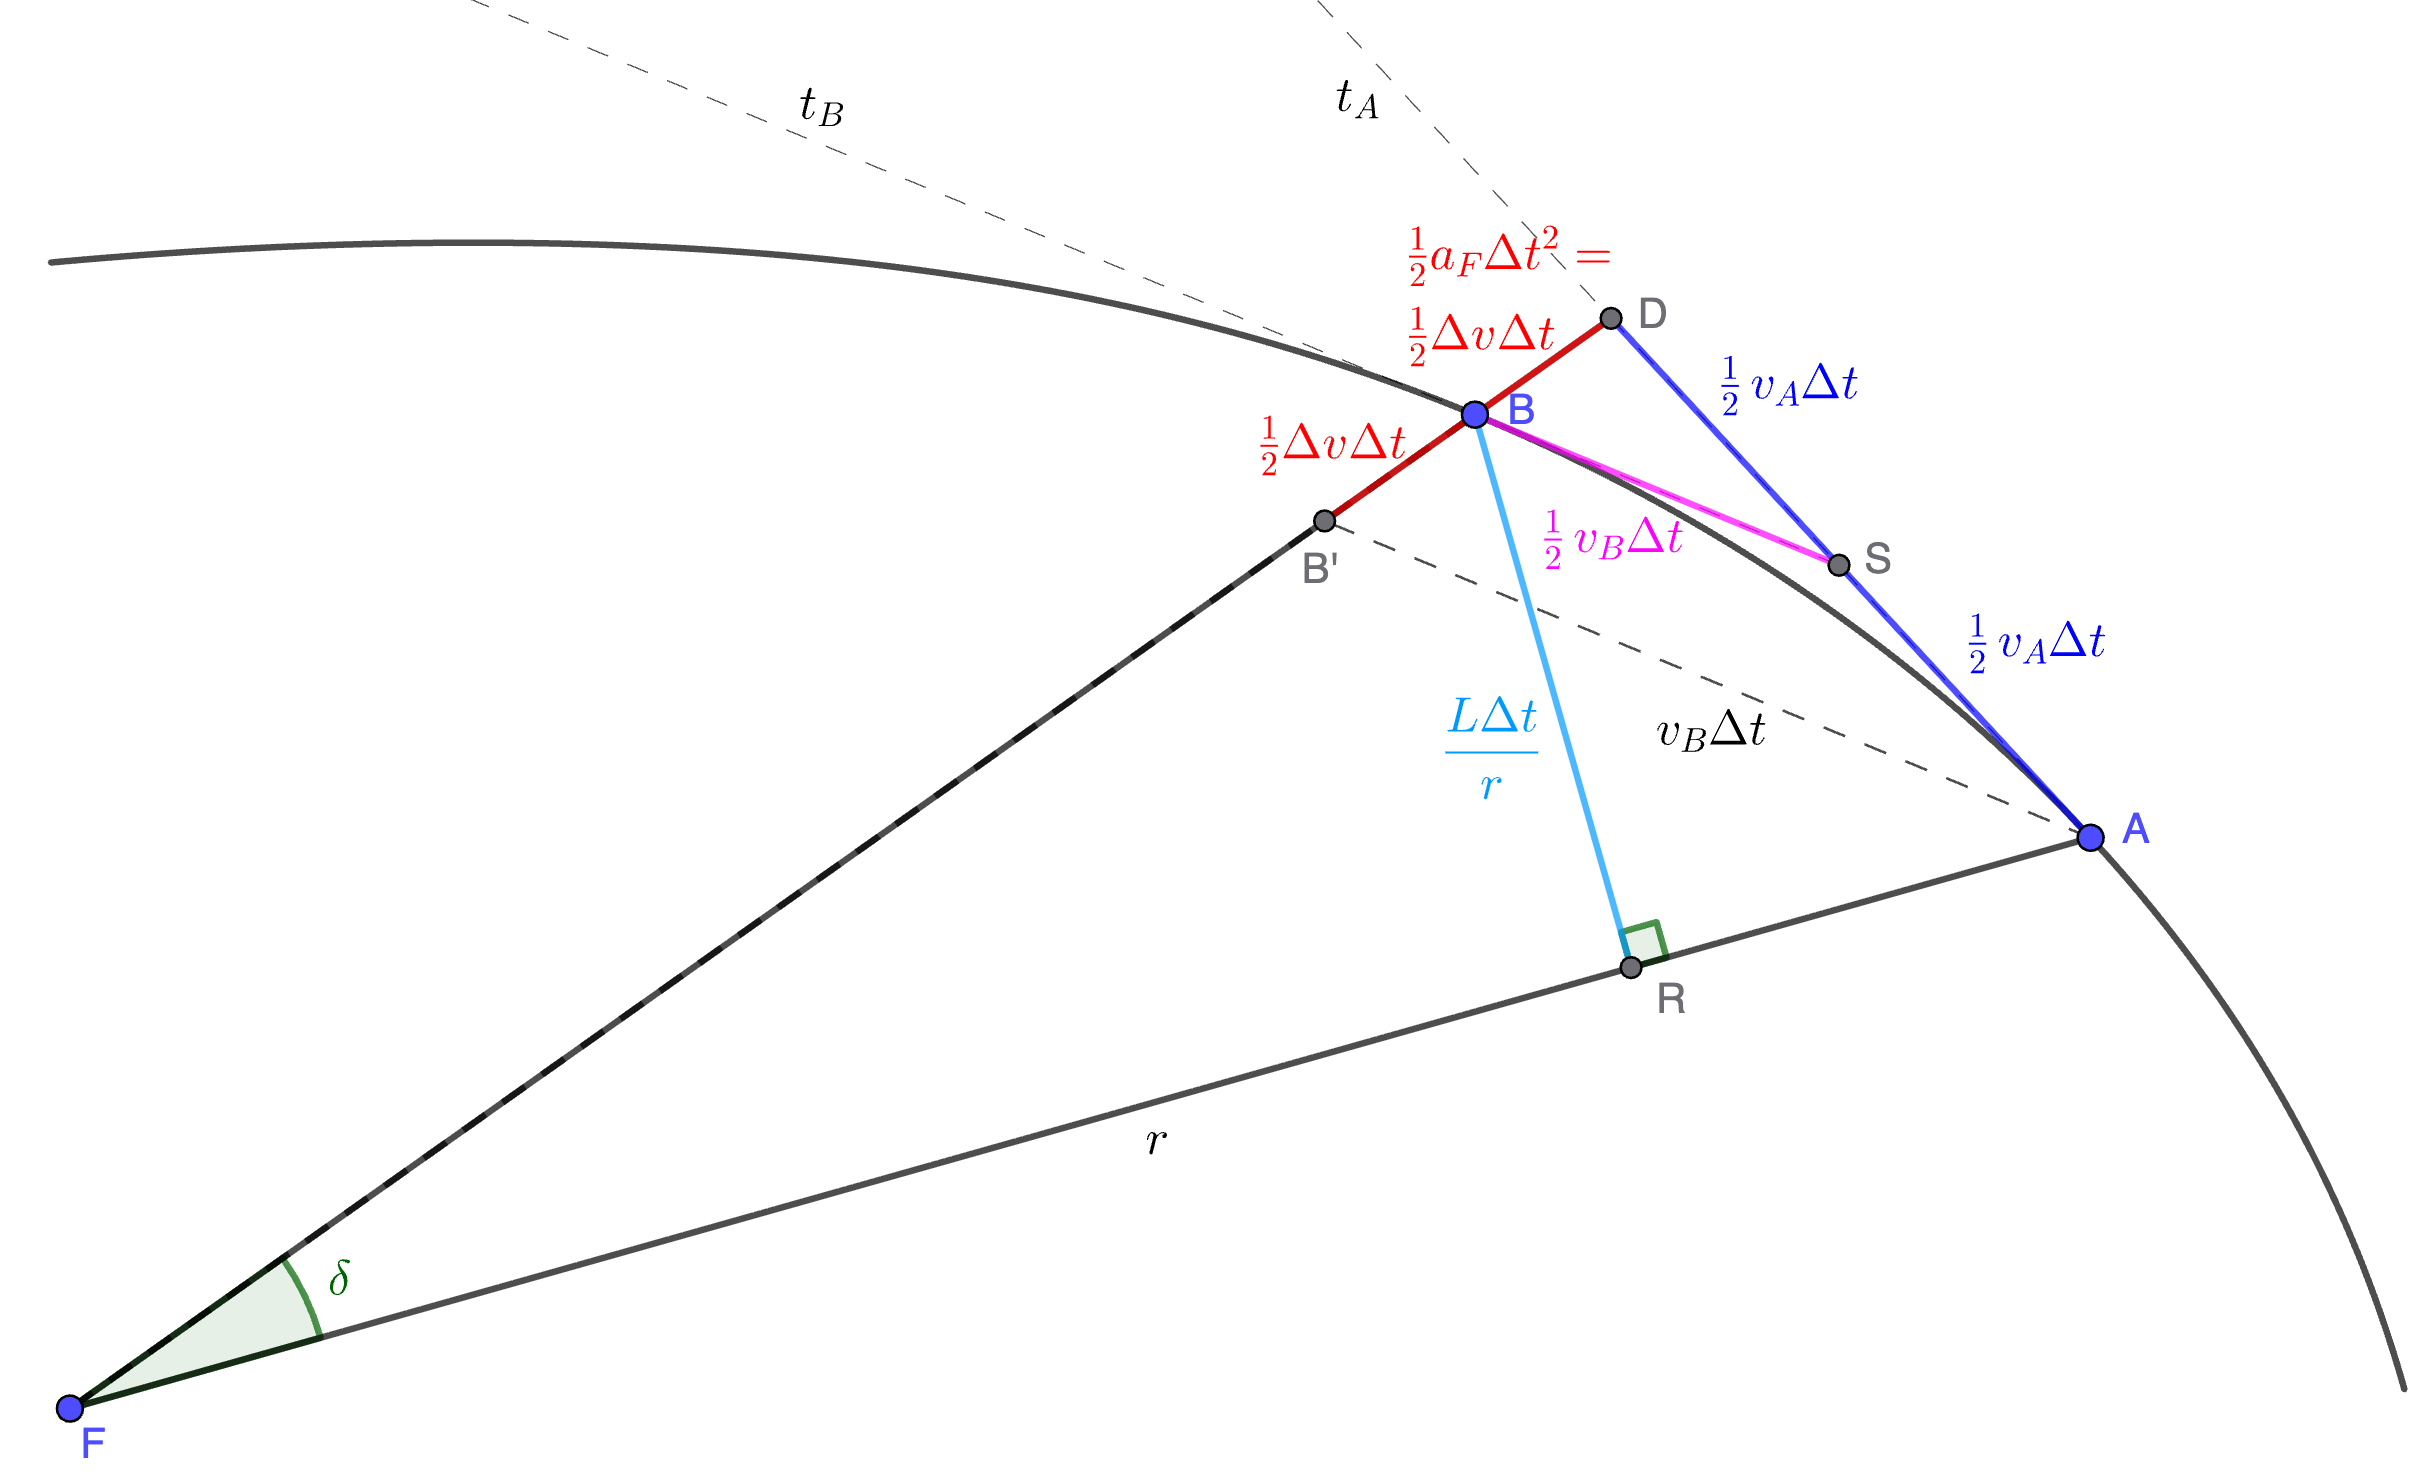
\includegraphics[width=1\linewidth]{assets/images/lemma_BD_BR2.png}
  \caption{Local construction used in \Cref{lem:deflection-identity,lem:bd-over-br2}.}
  \label{fig:lemma-bd-br2}
\end{figure}

\begin{lemma}[Deflection identity]
\label{lem:deflection-identity}
Over an evanescent time step $\Delta t$, the deflection produced by the mean acceleration $a_F$ satisfies
\begin{equation}
  BD=\frac12 a_F(\Delta t)^2=\frac12 \Delta v\,\Delta t,
  \qquad (\Delta v=a_F\Delta t).
\end{equation}
With the tangent construction, $S$ bisects $AD$; and in the limit $B\to A$,
\begin{equation}
  AS=SD=SB=\frac12\,\wideparen{AB}.
\end{equation}
\end{lemma}

\begin{proof}
From $\Delta v=a_F\Delta t$,
\[
  \frac12 a_F(\Delta t)^2
  =\frac12 (a_F\Delta t)\Delta t
  =\frac12 \Delta v\,\Delta t.
\]
Thus the deflection in time $\Delta t$ equals the distance generated by the mean velocity increment $\tfrac12\Delta v$ during $\Delta t$, namely the constructed segment $BD$. By construction, $S$ is the midpoint of $AD$, so $S$ bisects $AD$. As $B\to A$, the chordal midpoints coalesce in the ultimate ratio, giving
\[
  AS=SD=SB=\frac12\,\wideparen{AB}.
\]
\end{proof}

\begin{lemma}[Ratio \texorpdfstring{$BD/BR^2$}{BD over BR squared} and inverse-square form]
\label{lem:bd-over-br2}
Let $F$ be the center of force, $r=FB$, and $BR\perp FB$. Let $L$ be twice the areal speed, so
\[
  \Delta A=\frac{L}{2}\Delta t.
\]
Then, as $\Delta t\to 0$,
\begin{equation}
  BR\sim \frac{L\Delta t}{r},
  \qquad
  \frac{BD}{BR^2}\sim \frac12\,a_F\,\frac{r^2}{L^2}.
\end{equation}
Hence if $\dfrac{BD}{BR^2}\to c$, then
\begin{equation}
  a_F=\frac{2cL^2}{r^2},
  \qquad
  \vec{a}_F=-\frac{2cL^2}{r^2}\,\hat{r}.
\end{equation}
\end{lemma}

\begin{proof}
From Prop.~I (1846), swept areas are proportional to times; for an evanescent step,
\[
  \Delta A\sim \frac12 r\,BR.
\]
Using $\Delta A=\frac{L}{2}\Delta t$ gives
\[
  \frac{L}{2}\Delta t\sim \frac12 r\,BR
  \quad\Longrightarrow\quad
  BR\sim \frac{L\Delta t}{r}.
\]
By \Cref{lem:deflection-identity},
\[
  BD=\frac12 a_F(\Delta t)^2.
\]
Substitute $BR\sim L\Delta t/r$ to obtain
\[
  \frac{BD}{BR^2}
  \sim
  \frac{\frac12 a_F(\Delta t)^2}{(L\Delta t/r)^2}
  =
  \frac12\,a_F\,\frac{r^2}{L^2}.
\]
So if the ratio tends to $c$, then $a_F=2cL^2/r^2$, directed toward $F$, i.e.
\[
  \vec{a}_F=-\frac{2cL^2}{r^2}\,\hat{r}.
\]
\end{proof}
